%! Author = partsjoo
%! Date = 14.04.2023

\documentclass[12pt]{article} % here to clear compiler errors

%
% Tallinn University of Technology - bachelor, master thesis template for LaTeX
%
% Public version 1.2
% 2022 Updated by Karl Janson to match the new formatting guidelines
%
% Public Version 1.1
% 2019 Adjusted by Frank Korving for his Bachelor Thesis, with contributions from Sander Arnus
%
% Public version 1.0
% 2010 - 2013 Thijs Nugteren and Joos Buijs for Master Thesis
%
% THIS IS THE MAIN FILE (i.e. compile this file, compiling the others directly won't work)
%

\documentclass[12pt, a4paper]{report}

% all the other includes etc. are done in the thesis.sty file.
\usepackage{thesis}
\usepackage{ifthen}
\usepackage{datetime}

\renewcommand{\dateseparator}{.}

%%%%%%%%%%%%%%%%%%%%%%%%%%%%%%%%%%%%%%%%%%%%%%%%%%%%%%%%%%%%%
% NOTE:                                                     %
%%%%%%%%%%%%%%%%%%%%%%%%%%%%%%%%%%%%%%%%%%%%%%%%%%%%%%%%%%%%%
% * Content chapter files are located in "chapters" folder, %
%   included using the "chapters_main.tex" file             %
%                                                           %
% * Appendices are located in "appendices" folder,          %
%   included using the "appendices_main.tex" file           %
%%%%%%%%%%%%%%%%%%%%%%%%%%%%%%%%%%%%%%%%%%%%%%%%%%%%%%%%%%%%%

%%%%%%%%%%%%%%%%%%%%%%%%%%%%%%%%%%%%%%%%%%%%%%%%%%%%%%%%%%%%%
% The commands below need to be defined.                    %
% Estonian title page will be generated automatically       %
%%%%%%%%%%%%%%%%%%%%%%%%%%%%%%%%%%%%%%%%%%%%%%%%%%%%%%%%%%%%%
\newcommand{\doctitle}{Homework 1: CISO roadmap}
%\newcommand{\doctitleEst}{[Lõputöö pealkiri]} % Title in Estonian

% Choose one
\newcommand{\doctype}{Cyber Security Management (ITC8230)}

% Thesis author
\newcommand{\authorName}{Joosep Parts}
\newcommand{\studentcode}{221963IVCM}

% Main supervisor
\newcommand{\supervisor}{Kaido Kikkas}
\newcommand{\supervisortitle}{Ph.D.}

% Co-supervisor. If you have only one supervisor, leave it as it is
\newcommand{\cosupervisor}{[Co-Supervisor's Name]}
\newcommand{\cosupervisortitle}{[Academic degree]}

% Dates. Default to current current date.
% You can hard code a value by replacing the parameter with a text
% Year of publication (defaults to current year).
\newcommand{\Year}{\the\year{}}

% Signature date (defaults to today).
\newcommand{\signatureDate}{\ddmmyyyydate\today}

% PDF Metadata
\newcommand{\version}{0.1 version}
\newcommand{\keywords}{Cyber security, risk assessment, telepresence robotics}

% CUSTOM COMMANDS
% Abbreviations setup
\usepackage{acro}

\setlength\LTleft{18pt}  % Adjust the left margin
\setlength\LTpre{-6pt}   % Adjust the space above the table

\acsetup{
  list/template = longtable,
  list/heading = none,
  templates/colspec = {l@{\hspace{2cm}}l} % Adjust the space as needed
}

%! Author = partsjoo
%! Date = 14.04.2023


% Plotting setup
\usepackage{pgfplots}

% Table setup
\usepackage{array}


%%%%%%%%%%%%%%%%%%%%%%%%%%%%%%%%%%%%%%%%%%%%%%%%%%%%%%%%%%%%%
%            DO NOT EDIT BELOW THIS LINE                    %
%%%%%%%%%%%%%%%%%%%%%%%%%%%%%%%%%%%%%%%%%%%%%%%%%%%%%%%%%%%%%

\newcommand{\university}{TALLINN UNIVERSITY OF TECHNOLOGY}
\newcommand{\school}{School of Information Technologies}
\newcommand{\universityEst}{TALLINNA TEHNIKAÜLIKOOL}
\newcommand{\schoolEst}{Infotehnoloogia teaduskond}

% For Estonian title page generation
\newcommand{\meEst}[1]
{
  \ifthenelse{\equal{#1}{[Author name]}}{Joosep Parts}{\authorName}
}

\newcommand{\studentcodeEst}[1]
{
  \ifthenelse{\equal{#1}{[Student Code]}}{[Üliõpilaskood]}{\studentcode}
}

\newcommand{\doctypeEst}[1]
{
  \ifthenelse{\equal{#1}{[Bachelor's Thesis / Master's Thesis]}}{[Bakalaureusetöö / Magistritöö]}{}
  \ifthenelse{\equal{#1}{Bachelor's Thesis}}{Bakalaureusetöö}{}
  \ifthenelse{\equal{#1}{Master's Thesis}}{Magistritöö}{}
}

\newcommand{\supervisorEst}[1]
{
  \ifthenelse{\equal{#1}{[Supervisor's Name]}}{[Juhendaja nimi]}{\supervisor}
}
\newcommand{\supervisortitleEst}[1]
{
  \ifthenelse{\equal{#1}{[Academic degree]}}{[Teaduskraad]}{\supervisortitle}
}

%
% PDF settings
%
\hypersetup
{
  pdfauthor={\authorName},
  pdfsubject={\doctitle},
  pdfkeywords={\keywords}
}

%! Author = partsjoo
%! Date = 16.04.2023

\newcommand{\thesisTitle}{Cyber Security Risks of Telepresence Robots in Higher Education and Their Mitigation}
\newcommand{\thesisTitleEst}{Kaugosalusrobotite küberturvalisuse riskid kõrgharidussüsteemis ja nende vähendamine}
\newcommand{\thesisAuthor}{Joosep Parts}
\newcommand{\thesisSupervisor}{Kaido Kikkas}
\newcommand{\todayDate}{\today}
\newcommand{\thesisYear}{2023}
\newcommand{\thesisType}{Master's Thesis (21 ECTS)}
\newcommand{\thesisUniversity}{University of Tartu}
\newcommand{\thesisInstitute}{Institute of Computer Science}
\newcommand{\thesisDepartment}{Cybersecurity Curriculum}
\newcommand{\thesisCity}{Tartu}
\newcommand{\thesisKeywordsEng}{Cyber security, risk assessment, telepresence robotics}
\newcommand{\thesisKeywordsEst}{Küberturvalisus, riskianalüüs, kaugosalus robootika}
\newcommand{\thesisAbbreviations}{List of Abbreviations and Terms}
\newcommand{\thesisCERCSEng}{T120 System technology, computer technology}
\newcommand{\thesisCERCSEst}{T120 Süsteemitehnoloogia, arvutitehnoloogia}

%! Author = partsjoo
%! Date = 14.04.2023


\usepackage[backend=biber,
  bibstyle=ieee,
  citestyle=numeric-comp,
%  citestyle=ieee,
%  bibstyle=numeric,
  urldate=iso,
  seconds=true]{biblatex}
\usepackage{enumerate}
\usepackage{glossaries-extra}
\usepackage{aguplus}
\usepackage{cals} % here to clear compiler errors
\addbibresource{ref.bib}
\renewcommand*{\multicitedelim}{\addsemicolon\space} % use semicolon instead

\begin{document}

  %! Author = partsjoo
%! Date = 16.04.2023

\thispagestyle{empty}
\begin{center}

\large
{\thesisUniversity}\\
{\thesisInstitute}\\
{\thesisDepartment}\\

%\vspace*{\stretch{5}}
\vspace{45mm}

\Large {\thesisAuthor}

\vspace{4mm}
\large

\huge{Exam 31.05.2023} \\
\vspace{4mm}
\Large {Privacy-preserving Technologies LTAT.04.007}


%\vspace*{\stretch{7}}
\vspace{20mm}

%\Large {\thesisType}

\end{center}

\vspace{2mm}

\begin{flushright}
 {
 \setlength{\extrarowheight}{5pt}
 \begin{tabular}{r l} 
%  \sffamily Supervisor: {\thesisSupervisor}, PhD
 \end{tabular}
 }
\end{flushright}

%\vspace*{\stretch{3}}\iflanguage
%\vspace{10mm}

\vfill
\centerline{\large {\thesisCity} {\thesisYear}}

%===END TITLE PAGE



  \newpage
  \clearpage
  \phantomsection
  \printacronyms

  \newpage
  \tableofcontents


  %! Author = partsjoo
%! Date = 14.04.2023

\newpage


\section{Analysis}

Before choosing any options the given set was pre-analyzed using analyze utility to determine the \ac{SA} of the set.
Anonymization options were redefined during the process many times to yeild desired result, but for the baseline settings the first chosen
settings were synthesised quite subjectively. Data set is a sample set of COVID-19 health related data, see Figure~\ref{fig:my_label3}
for example.

\begin{figure}[ht]
  \centering
  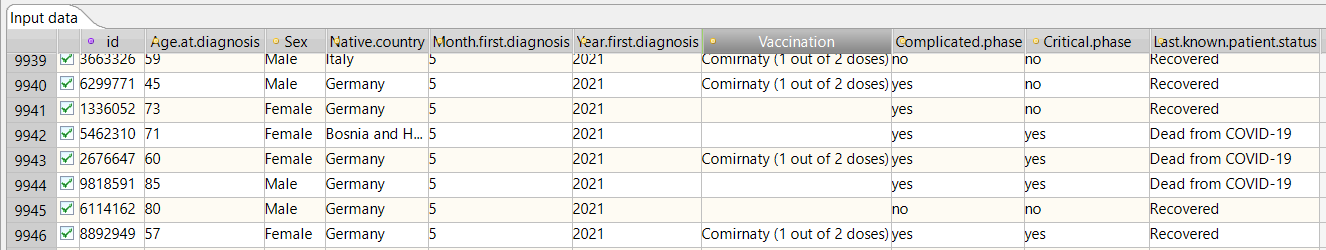
\includegraphics[width=\textwidth, keepaspectratio]{assets/sample_data}
  \caption{Preview of the sample set}
  \label{fig:my_label3}
\end{figure}

\subsection{Levels of generalisation}

Before choosing levels of generalisation all fields distribution was observed to determine possible ways to generalisation. For example
countries distribution was observed in Figure~\ref{fig:my_label1} and it was seen that smaller countries should be concatenated due to their
small sample size. And from observing age (see Figure~\ref{fig:my_label2}), I saw that most records existed for older ages, so
it
would make sense to
group younger and middle-aged people wider than the older ages. Few fields were not generalised. If we transformed all the values of the
given set we would lose the context greatly making the output data quite useless. Since we dont know what the \ac{DS} may not wish to be
disclosed explicitly, I have not generalised some \ac{DA}, see Table~\ref{tab:table2}. But for other \ac{DA} following suggestions for
data anonymization
as relevant guidelines suggest on doing~\cite[]{www.operando.eu}.

\begin{figure}[ht]
  \centering
  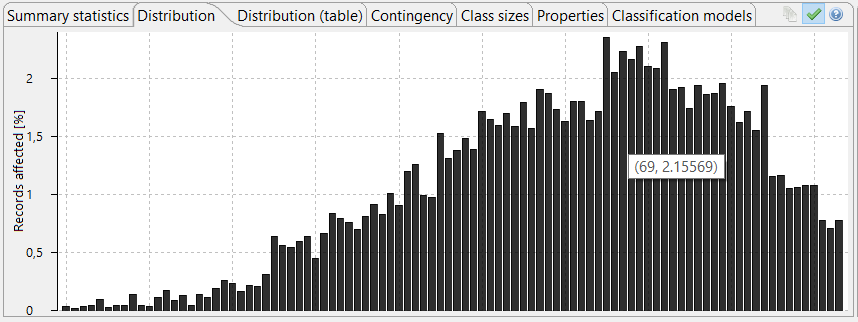
\includegraphics[width=\textwidth, keepaspectratio]{assets/age_dist}
  \caption{Initial age distribution}
  \label{fig:my_label2}
\end{figure}

\begin{figure}[ht]
  \centering
  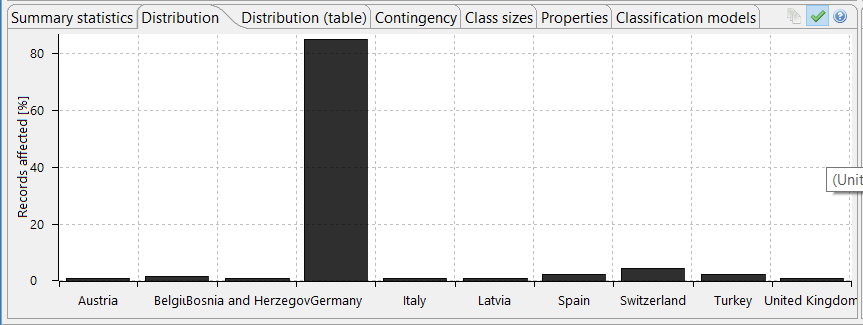
\includegraphics[width=\textwidth, keepaspectratio]{assets/countries_dist}
  \caption{Initial countries distribution}
  \label{fig:my_label1}
\end{figure}

\begin{table}[ht]
  \small
  \centering
  \caption{Chosen Generalizations}
  \begin{tabular}{lll}
    \toprule
    \textbf{Generalization}      & \textbf{Levels} & \textbf{Field}            \\
    \midrule
    --                           & Level 1         & id                        \\
    Intervals (5y)               & 6 levels        & Age.at.diagnosis          \\
    Ordering                     & 1 levels        & Sex                       \\
    Priority grouping descending & 3 levels        & Native.country            \\
    --                           & --              & Month.first.diagnosis     \\
    Intervals                    & 2 levels        & Year.first.diagnosis      \\
    Priority grouping            & 3 levels        & Vaccination               \\
    --                           & --              & Complicated.phase         \\
    --                           & --              & Critical.phase            \\
    Priority grouping            & 3 levels        & Last.known.patient.status \\
    \bottomrule
  \end{tabular}\label{tab:table2}
\end{table}

As seen in Table~\ref{tab:table2}, for the ``id`` field, a single level of generalisation is applied to suppress or replace all unique
identifiers, thus
providing
strong privacy protection. Age at diagnosis, a quasi-identifier, is divided into 5-year intervals with 6 levels to maintain data utility
while reducing the risk of re-identification. A 5-year range is a common choice in literature~\cite[672]{el2009globally}, as it achieves a balance between privacy
and utility. I would have wanted to group lower and middle aged people in a wider range than older ages, but I could not find the options
to do so.
To
minimize the risk of re-identification for the
``Sex``
attribute without significantly affecting data utility, we group genders while preserving their distribution.

For the ``Native.country`` field, we employ priority grouping with three descending levels based on factors such as geography or demographics to ensure sufficient generalization without excessive information loss. The ``Month.first.diagnosis`` attribute is not generalized, preserving its full utility under the assumption that the month of diagnosis alone does not significantly contribute to re-identification risk when combined with other anonymized attributes.

The ``Year.first.diagnosis`` attribute is generalised using intervals with two levels, while the ``Vaccination`` and ``Last.known.patient.status`` fields are subjected to priority grouping with three levels, ensuring a balance between privacy protection and data utility. Finally, no generalization is applied to the ``Complicated.phase`` and ``Critical.phase`` attributes, as they are deemed not to significantly increase re-identification risk in combination with other anonymized attributes

\subsection{Guarantees the privacy models offer}\label{subsec:guarantees-the-privacy-models-offer}

When analyzing data to anonymize using the ARX tool, I chose to use k-anonymity with k=5 and l-distinct 10-diversity to ensure privacy
and data utility.

K-anonymity is a privacy model that aims to protect individual identities in a dataset by ensuring that each record cannot be uniquely
distinguished from at least k-1 other records~\cite[]{sweeney2002k}.
When k-anonymity is set to 5, it means that for any given
combination of quasi
-identifiers (attributes that can be used to identify individuals indirectly) in the dataset, there are at least five records with the same
values.
L-distinct diversity is a privacy model that extends k-anonymity by ensuring diversity in sensitive attributes within each group
of records sharing the same quasi-identifiers.
This helps protect against attribute disclosure, where an attacker could infer sensitive
information about an individual even if their identity is not revealed~\cite[]{sweeney2002k}.
Applying both helps to prevent the re
-identification of individuals in the dataset.
Because we had id in out set L-distinct diversity was required by ARX.

A higher value of k-anonymity or L-distinct diversity would provide more privacy, but lead to a significant loss of data utility due to generalisation or suppression
while
lower levels didn't provide enough protection.
So I tested with ranges from 2..10 and ended up somwhere in middle of k=5 and l=10. \ac{ico}

\begin{figure}[ht]
  \smaller
  \centering
  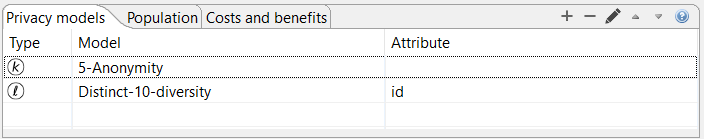
\includegraphics[width=\textwidth, keepaspectratio]{assets/anon_level}
  \caption{Applied privacy models}
  \label{fig:my_label}
\end{figure}

\subsection{Chosen transformations and levels}\label{subsec:chosen-transformations-and-levels}

``id`` is a sensitive attribute because it represents a unique identifier for each individual in the dataset. Protecting this attribute
is critical, as it can directly lead to the re-identification of individuals. Other attributes on their own might not be sufficient to
uniquely identify individuals, but when combined, they can increase the risk of
re-identification. By treating them as quasi-identifiers, I reduce this risk and ensure that the ARX tool considers them when applying
privacy models like k-anonymity and l-diversity~\cite[]{arx}. This approach allows me to apply different levels of privacy protection.

\begin{table}[ht]
  \small
  \centering
  \caption{Chosen data transformation types}
  \begin{tabular}{cl}
    \toprule
    \textbf{Sensitive Attributes} & \textbf{Quasi-identifiers} \\
    \midrule
    id                            & Age.at.diagnosis           \\
    & Sex                        \\
    & Native.country             \\
    & Month.first.diagnosis      \\
    & Year.first.diagnosis       \\
    & Vaccination                \\
    & Complicated.phase          \\
    & Critical.phase             \\
    & Last.known.patient.status  \\
    \bottomrule
  \end{tabular}\label{tab:table}
\end{table}

\subsection{Minimal class size and number of records suppressed}

\begin{figure}[ht]
  \centering

  \begin{subfigure}{0.49\textwidth}
    \centering
    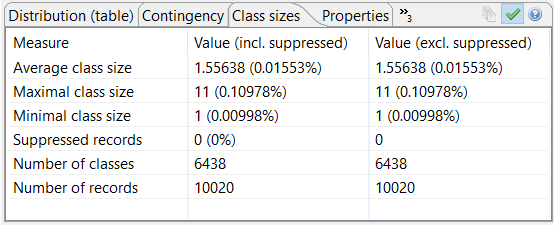
\includegraphics[width=\linewidth]{assets/class_size_unsupressed}
    \caption{Class size unsuppressed}
    \label{fig:subim1}
  \end{subfigure}
  \hfill
  \begin{subfigure}{0.49\textwidth}
    \centering
    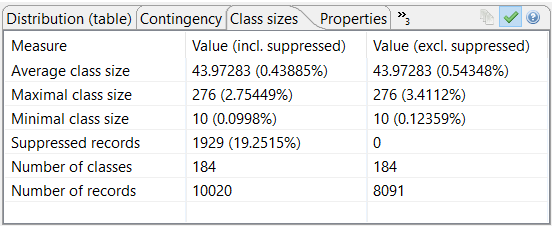
\includegraphics[width=\linewidth]{assets/class_size_supressed}
    \caption{Class size suppressed}
    \label{fig:subim2}
  \end{subfigure}

  \caption{Class size suppressions before and after}
  \label{fig:image2}
\end{figure}

Figure~\ref{fig:image2} shows class sizes before and after anonymization. Prior to anonymization, the dataset comprised 10,020 records with no suppressed records as seen on Figure~\ref{fig:subim1}. The average
class size was 1
.55638 (0.01553\%), with a maximal class size of 11 (0.10978\%) and a minimal class size of 1 (0.00998\%). There were 6,438 classes in total.
In Figure~\ref{fig:subim2}, after anonymization process, the dataset contained 8,091 records, with 1,929 (19
.2515\%) records
suppressed. The
average
class
size increased to 43.92283 (0.43885\%), with a maximal class size of 226 (3.4112\%) and a minimal class size of 10 (0.0998\%). The total number of classes reduced to 184.

The comparison of the dataset before and after anonymization reveals a significant change in the distribution of records. The number of suppressed records increased to 1,929 (19.2515\%), indicating a stronger emphasis on privacy protection. This increase in suppression, however, comes at the cost of data utility, as more records are removed from the dataset.

The average class size grew substantially from 1.55638 (0.01553\%) to 43.92283 (0.43885\%), reflecting the generalisation applied to the attributes. This generalisation ensures that each group of records sharing the same quasi-identifiers has a higher level of anonymity, but it may also lead to a loss of granularity in the data.

The maximal and minimal class sizes also changed considerably after anonymization. The maximal class size increased from 11 (0.10978\%) to 226 (3.4112\%), while the minimal class size rose from 1 (0.00998\%) to 10 (0.0998\%). These changes highlight the impact of the anonymization techniques in creating a more uniform distribution of records across classes, enhancing privacy protection.

Quality models as seen in Figure~\ref{fig:my_label5} interestingly show that ``Age.at.diagnosis`` was considered the most revealing and
was completely suppressed in the output data while other~\ac{DA} remained in the near 20\% range.

\begin{figure}[ht]
  \smaller
  \centering
  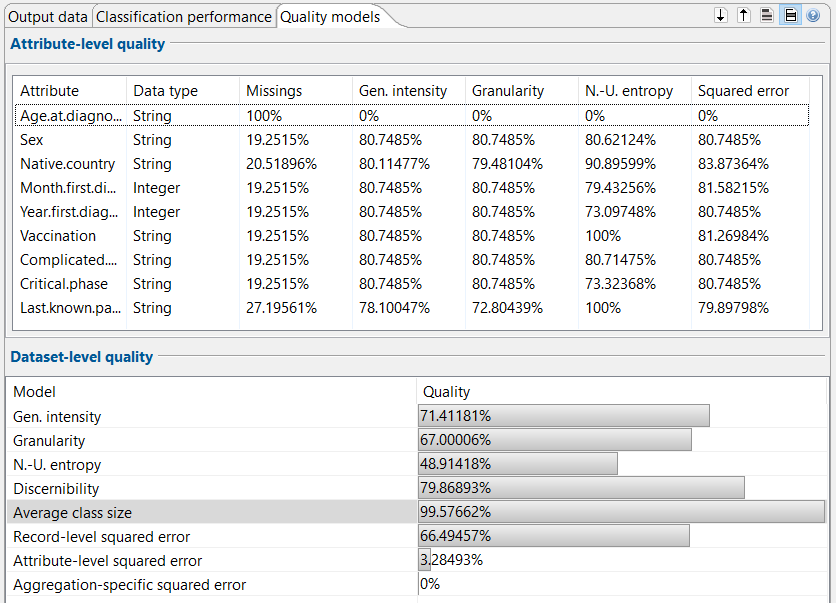
\includegraphics[width=300pt, keepaspectratio]{assets/quality_models}
  \caption{Quality models after anaonmization}
  \label{fig:my_label5}
\end{figure}


In summary, it can be reasonably concluded that appropriate measures have been taken to anonymize the dataset in question. Although it is
essential
to further evaluate the sufficiency of the generalisations applied, such an assessment is contingent upon the specific context in which the data is required, the stipulated data constraints, and any~\ac{DA} suppression that may be explicitly requested by the~\ac{DS}. Given the scope of this exercise, the output generated is adequate in demonstrating the effectiveness of the anonymization process. For a visual representation of the results, please refer to Figure~\ref{fig:my_label4}.


\begin{figure}[ht]
  \smaller
  \centering
  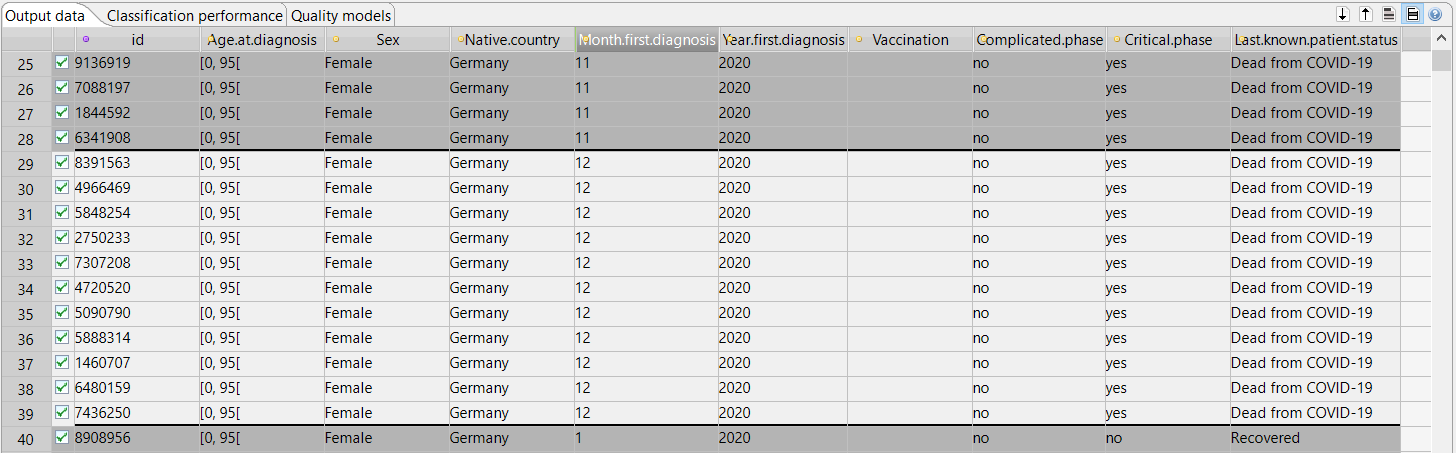
\includegraphics[width=\textwidth, keepaspectratio]{assets/data_out}
  \caption{Output dataset after anonymization process}
  \label{fig:my_label4}
\end{figure}

\clearpage
\newpage

\subsection{Risk of the input data and output data}

\begin{figure}[ht]
  \smaller
  \centering
  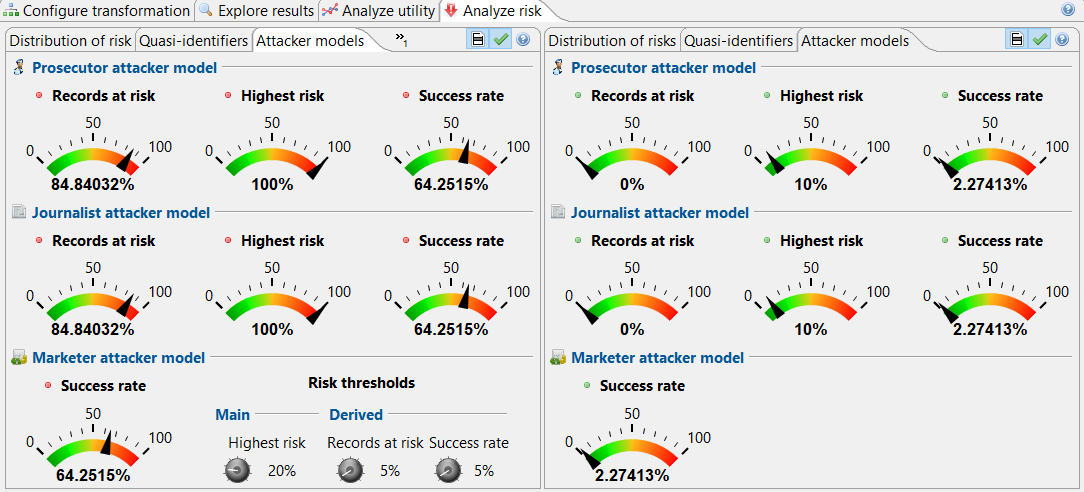
\includegraphics[width=\textwidth, keepaspectratio]{assets/risk_meter}
  \caption{Attcker model risk meters}
  \label{fig:my_label6}
\end{figure}

\begin{figure}[ht]
  \centering

  \begin{subfigure}{0.49\textwidth}
    \centering
    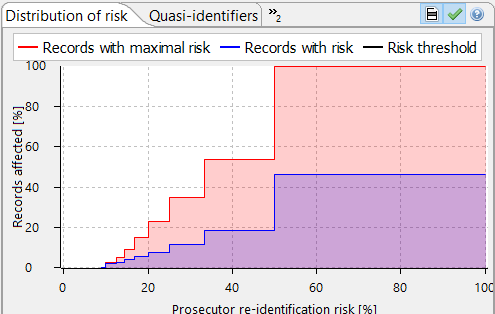
\includegraphics[width=\linewidth]{assets/risk_before}
    \caption{Risk analyzis before ananymization}
    \label{fig:subim3}
  \end{subfigure}
  \hfill
  \begin{subfigure}{0.49\textwidth}
    \centering
    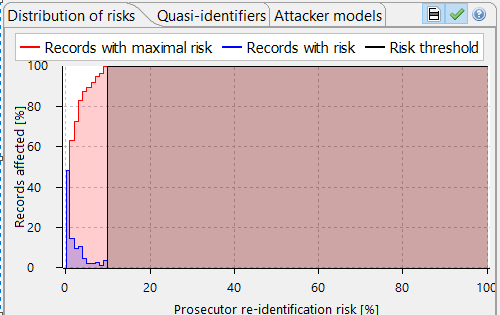
\includegraphics[width=\linewidth]{assets/risk_after}
    \caption{Risk analyzis after ananymization}
    \label{fig:subim4}
  \end{subfigure}

  \caption{Risk before and after}
  \label{fig:image3}
\end{figure}

The risk analysis conducted before and after data anonymization provides valuable insights into the effectiveness of the anonymization
process in mitigating privacy risks associated with various types of adversaries, such as prosecutors, journalists, and marketers. Before
anonymization on Figure~\ref{fig:subim3} and looking at risk metrics on Figure~\ref{fig:my_label6} we can see that about 60-80\% of our
records are at high risk and records are identifiable by different models. Which is not suprising none of the~\ac{DA} are supressed. Yet
which is surprising, is that even with ``id`` fields given the percent is not 100\% which I found odd. In the other hand, after
ananomyzation, we can see that on all attacker models out records are relatively safe with the highest risk being around 10\% with
marginal 2\% success rate.



  \newpage
  \newpage
  \printbibliography


\end{document}
